\documentclass[a4paper]{article}

\usepackage{acronym}
\usepackage[intoc]{nomencl}
\usepackage{todonotes}
\usepackage{listings}
\usepackage{color}
\usepackage{amsmath}
\usepackage{amsfonts}
\usepackage{acronym}
\usepackage{bytefield}
\usepackage{marvosym}
\usepackage[pdftex,
		pdfauthor={Roel Baardman},
		pdftitle={Transponder check}]{hyperref}
		


\definecolor{dkgreen}{rgb}{0,0.6,0}
\definecolor{gray}{rgb}{0.5,0.5,0.5}
\definecolor{mauve}{rgb}{0.58,0,0.82}

\lstset{	keywordstyle=\color{blue},
		commentstyle=\color{dkgreen},
		stringstyle=\color{mauve},
		numbers=left,
		numberstyle=\tiny\color{gray},
		stepnumber=2,
		numbersep=5pt,
		breaklines=true,
		breakatwhitespace=false,
		title=\lstname
}


\graphicspath{{img/}}

%\renewcommand*{\pagedeclaration}[1]
%{
%	\unskip
%	, page \hyperpage{#1}
%}

%Derivative
\newcommand{\derivative}[2]
{
	\frac{\partial #1}{\partial #2}
}

%Scientific notation
\newcommand{\e}[1]{\ensuremath{\times 10^{#1}}}

%Checklist commands
\newcommand{\itemcheck}[1]
{
        \item[\Squarepipe]{#1}
}

\newcommand{\itemchecked}[2]
{
        \item[\Checkedbox]{#1}
        \emph{#2}
}

\newcommand{\itemfailed}[2]
{
        \item[\Info]{#1}
        \emph{#2}
}

%These are derived from ISO-1151
\newcommand{\angleofattack}
{
	\alpha
}

\newcommand{\angleofsideslip}
{
	\beta
}

\newcommand{\azimuth}
{
	\Psi
}

\newcommand{\inclination}
{
	\Theta
}

\newcommand{\bankangle}
{
	\Phi
}

\newcommand{\angularvelocity}
{
	\Omega
}

\newcommand{\mach}
{
	Ma
}

%Quaternions
\newcommand{\quaternion}[4] {
\begin{bmatrix}
#4 \\
#1 \\
#2 \\
#3 \\
\end{bmatrix}
}

%Statistics
\newcommand{\stdev}
{
	\sigma
}

\newcommand{\variance}
{
	\sigma^2
}

%Misc
\newcommand{\nomen}[3]
{
	\nomenclature{#1}{#2 \hfill\makebox[8em]{#3\hfill}}
	Where #1 is the #2 (#3). \\
}

\newcommand{\myquote}[1]
{
	\textit{#1}
}

\newcommand{\chapterref}[1]
{
	Chapter \ref{chap:#1}
}

\newcommand{\chapterlabel}[1]
{
	\label{chap:#1}
}

\newcommand{\labeledchapter}[2]
{
	\chapter{#1}
	\chapterlabel{#2}
}

\newcommand{\sectionref}[1]
{
	Section \ref{sec:#1}
}

\newcommand{\sectionlabel}[1]
{
	\label{sec:#1}
}

\newcommand{\labeledsection}[2]
{
	\section{#1}
	\sectionlabel{#2}
}

\newcommand{\figureref}[1]
{
	Figure \ref{fig:#1}
}

\newcommand{\figurelabel}[1]
{
	\label{fig:#1}
}

\newcommand{\tableref}[1]
{
	Table \ref{tab:#1}
}

\newcommand{\equationref}[1]
{
	Equation \ref{eq:#1}
}

\newcommand{\equationlabel}[1]
{
	\label{eq:#1}
}

\newcommand{\listingref}[1]
{
	Code Listing \ref{lst:#1}
}



\begin{document}
\section{Source documents}
\subsection{Aircraft Maintainance Program}
The maintainance manual of PH-1516\cite{AMP_PH1516} references MD NL-2011-002 R1, due to the existance of a transponder installation.

\subsection{Maintainance Directive}
\subsubsection{Appendix A}
The Dutch government writes in MD NL-2011-002 R1\cite{NL_2011_002_R1}, Appendix A, Table 1, Footnote 3: \texttt{``Refer to EC Regulation 1207/2011 article 7(2) for mandatory periodic testing of Mode S Transponder systems.''}
\subsubsection{Appendix B}
The Dutch government writes in MD NL-2011-002 R1\cite{NL_2011_002_R1}, Appendix B, Point 4: \texttt{``Operational checking of the transponder is required, as part of the radio identification equipment check. Maintenance tests should include a periodic verification check of aircraft derived data including the ICAO 24 bit aircraft address using suitable ramp test equipment1. For this transponder operational check, please follow the instructions in EASA SIB 2011-15, Appendix 1, which are provided to minimise the hinder such testing causes to air traffic control [...]''}

\subsection{{EC} Regulation}
\subsubsection{Article 7(2)}
EC Regulation 1207/2011\cite{EC_1207_2011} article 7(2) states: \texttt{``Operators shall ensure that a check is performed at least every two years, and, whenever an anomaly is detected on a specific aircraft, so that the data items set out in point 3 of Part A of Annex II, in point 3 of Part B of Annex II and in point 2 of Part C of Annex II, if applicable, are correctly provided at the output of secondary surveillance radar transponders installed on board their aircraft. If any of the data items are not correctly provided then the operator shall investigate the matter before the next flight is initiated and any rectification necessary shall be introduced in line with normal maintenance and corrective procedures for the aircraft and its avionics.''}
\subsubsection{{Annex II, Part A}}
Point 3, applicable for Mode-S transponders, lists these items:
\begin{itemize}
\item[a]{24-bit ICAO aircraft address}
\item[b]{Mode A code}
\item[c]{Pressure altitude}
\item[d]{Flight status (on the ground or airborne)}
\item[e]{Data link capability report}
\item[f]{Common usage {GICB} capability report}
\item[g]{Aircraft identification}
\item[h]{Special position indication (SPI)}
\item[i]{Emergency status}
\item[j]{{ACAS} active resolution advisories when the aircraft is equipped with TCAS II}
\end{itemize}

\subsection{{EASA} Safety Information Bulletin}
EASA SIB 2011-15R2\cite{EASA_SIB_2011_15R2}, Appendix 1 states:
\begin{itemize}
\item[a.]{When not required, ensure all transponders are selected to ‘OFF’ or ‘Standby’.}
\item[b.]{Before starting any test, contact the local Air Traffic Control Unit and advise them of your intention to conduct transponder testing. Advise the Air Traffic Unit of your start time and test duration. Also inform them of the altitude(s) at which you will be testing, your intended Aircraft Identification (Flight Id) and your intended Mode A code. See para c and d. Note: Certain altitudes may not be possible due to over flying aircraft.}
\item[c.]{Set the Mode A code to 7776 (or other Mode A code agreed with Air Traffic Control Unit). Note: The Mode A code 7776 is assigned as a test code by the ORCAM Users Group, specifically for the testing of transponders.}
\item[d.]{For Mode S equipped aircraft, set the Aircraft Identification (Flight Id) with the first 8 characters of the company name. This is the name of the company conducting the tests.}
\item[e.]{For Mode S equipped aircraft, set the on-the-ground status for all Mode S replies, except when an airborne reply is required (e.g. for altitude testing).}
\item[f.]{Where possible, perform the testing inside a hanger to take advantage of any shielding properties it may provide.}
\item[g.]{As a precaution, use antenna transmission covers whether or not testing is performed inside or outside.}
\item[h.]{When testing the altitude (Mode C or S) parameter, radiate directly into the ramp test set via the prescribed attenuator.}
\item[i.]{In between testing, i.e. to transition from one altitude to another, select the transponder to ‘standby’ mode.}
\item[j.]{If testing transponder parameters other than ‘altitude’, set altitude to -1000 feet (minus 1000 feet), or over 60000 feet. This will minimise the possibility of ACAS warning to airfield and overflying aircraft.}
\item[k.]{When testing is complete select the transponder(s) to ‘OFF’ or ‘Standby’.}
\end{itemize}

\section{Test protocol}

\begin{enumerate}
\item Place the aircraft under test inside a hangar. Place the aircraft such that the wingtips are at the same height and the aircraft is in balance.
\item Power the transponder under test on, switch it to ``Standby'' mode.
\item Request the aerodrome's QNH and write it down.
\item Start the command \texttt{{rtl\_sdr -f 1090000000 -s 2000000 -g 50 - | pv -cN output > output.bin}} and verify that data is flowing at more than 3MegaBytes per second.
\item Note the time (on the computer) the command was started.
\item Switch the transponder under test from ``Standby'' to ``Alt''.
\item Note the time (on the computer) the transponder was started.
\item Measure the transponder for a full minute.
\item Switch the transponder from ``Alt'' back to ``Standby''.
\item Note the time (on the computer) the transponder was switched back.
\end{enumerate}

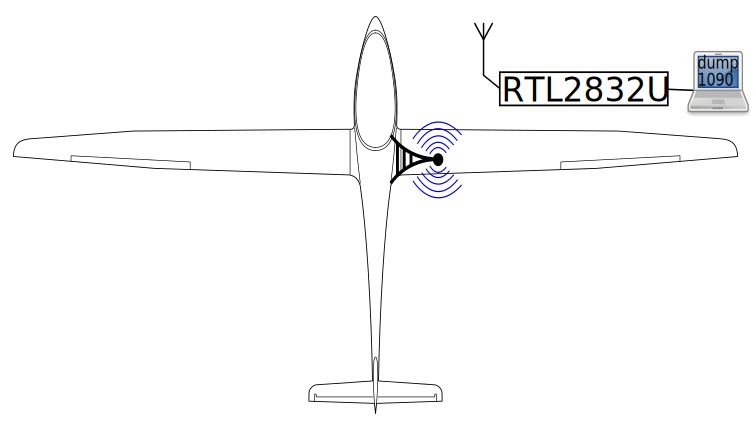
\includegraphics[width=\textwidth]{setup}

\bibliographystyle{ieeetr}
\bibliography{references}


\end{document}
